\chapter{Assignment \#9: PWR Loss of Coolant Containment Analysis}
\label{ch:ass9}


\begin{fullwidth}
\section{Background}
To prevent the release of radioactive fission products to the environment, reactor systems are protected with multiple barriers.  For light water reactors (LWRs) these barriers include the fuel material, the cladding around the fuel pins along with the reactor coolant system piping itself.  Since, for LWRs, the reactor coolant system is highly pressurized, it is possible that radioactive materaials may not be fully controlled due to failure of the reactor coolant pressure boundary.  For this reason, the reactor coolant systems for LWRs are surrounded by a larger \emph{containment building.}
\begin{figure}
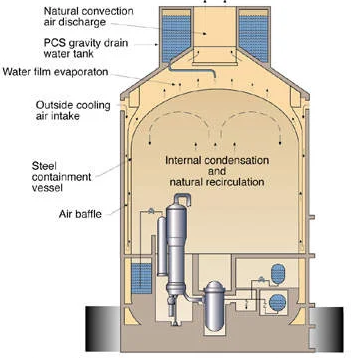
\includegraphics[width=7.50cm]{AP1000-containment.png}
\caption{AP1000 containment building}
\end{figure}
\newthought{What is not} so clear from the figure above is that the containment vessel must serve purposes beyond that strictly required for exclusion of fission products from the environment; the containment must be large enough to accomodate refueling equipment and allow for accessibility of major reactor plant components among other design requirements.

\newthought{In this workshop} we will practice the skills that will allow us to answer the question: if all of the primary coolant were released from the reactor coolant system into the containment; what would the resulting temperature and pressure be?  Of course to do this we will need to know some details about the design parameters of the primary coolant system and the containment; we will also need to make some reasonable assumptions to simplify the analysis. 

Initially, we will only require knowledge of the temperature, pressure and volume of the reactor coolant system and containment vessel.  We will assume that the air in the containment has negligible moisture content.  The primary coolant escaping from the reactor coolant system will expand to fill the total volume---volume of reactor coolant system plus the volume of the containment---and come into thermal equilibrium with the air.  We will assume that this process happens instantaneously and that there is no further heat input from the core (due, for example, to decay heat) or energy lost from the system due to heat transfer through the containment walls.

The conservation of energy equation for these assumptions reduces to the following:
$$m_w\left(u_{w_2} - u_{w_1}\right) + m_a\left(u_{a_2} - u_{a_1} \right) = Q_{1 \rightarrow 2} $$
We will assume that the total system volume remains constant:
$$V_{\text{final}} = V_{\text{containment}} + V_{\text{reactor coolant}}$$
where initially the air occupies $V_{\text{containment}}$ and the reactor coolant occupies $V_{\text{reactor coolant}}$.  The total system pressure is the sum of the partial pressures of the air and the primary coolant at the final temperature
$$P_{\text{final}} = P_{\text{air,final}} + P_{\text{water,final}}$$
with the air and water in thermal equilibrium---i.e. $T_{\text{air,final}} = T_{\text{water,final}}$.

\section{Part 1}

We will carry out the analysis to determine final containment volume pressure and temperature following a loss of coolant accident.  Relevant design information is provided in the table below.

\begin{table}
\begin{tabular}{l | l | l | l}
\toprule
\textbf{Component} & \textbf{Volume (m$^3$)} & \textbf{Pressure (kPa)} & \textbf{Temperature ($^{\circ}$C)} \\
\hline
Reactor coolant system & 354 & 15,500 & 340 \\
\hline
Containment vessel air & 50,970 & 101 & 27 \\
\bottomrule
\end{tabular}
\end{table}

\newthought{Consider a loss} of coolant accident where there is no heat added (for example, due to decay heat) and no heat lost (for example, via the containment shell to the atmosphere).  Answer the questions below:

\begin{enumerate}
\item What is the final containment temperature? [$^{\circ}$C]
\vspace{1.0 cm}
\item What is the partial pressure of water vapor in the containment? [kPa]
\vspace{1.0 cm}
\item What is the partial pressure of air in the containment? [kPa]
\end{enumerate}

\section{Part 2}
In the previous section we assumed that there would be no further heat input following the LOCA.  Due to the presence of decay heat, this assumption is both incorrect and non-conservative.  Over time, we can expect the pressure and temperature within the containment to increase due to heat input from the decay of fission products.  We also assumed for simplicity that the structure and shielding components within the containment volume have negligible heat capacity and that there are no other sources of water to cool the core in the case of an accident.  For this part of the assignment we will take into account heat input due to decay heat.  We will also account for the presence of emergency water sources such as the core make-up tanks and the irradiated water storage tank.

\begin{table}
\begin{tabular}{l | l | l | l}
\toprule
\textbf{Component} & \textbf{Volume (m$^3$)} & \textbf{Pressure (kPa)} & \textbf{Temperature ($^{\circ}$C)} \\
\hline
Irradiated water storage tank & 2,070 & 101 & 27 \\
\hline
Core make-up tanks & 141 & 101 & 27 \\
\bottomrule
\end{tabular}
\end{table}
The heat input due to decay heat can be approximated as follows:
$$P(t) = 0.066P_o\left[t^{-0.2}-(t+t_s)^{-2} \right]$$
where $P_o$ is the average power at which the reactor was operating prior to the accident, $t$ is the time since shutdown (in seconds, assuming the reactor was shutdown at the beginning of the LOCA); and $t_s$ is the duration of time that the reactor was previously operating before the shutdown (in seconds).  For this problem assume that the reactor was operating at 3400 MW$_{\text{th}}$ for a full year prior to the loss of coolant accident.

\begin{enumerate}[resume]
\item What is the final containment pressure and temperature at the end of one day?

\vspace{1.0 cm}

\item Make a plot of containment pressure and temperature from one second after the LOCA through one full day.  


\end{enumerate}


\end{fullwidth}
